\documentclass{article}
\usepackage[english]{babel}
\usepackage{cancel}
\usepackage{tikz}
\usepackage{amsmath}
\usepackage{amsfonts}
\usepackage{amssymb}
\usepackage{graphicx}
\usepackage{subcaption}
\usepackage{caption}
\usepackage{hyperref}
\graphicspath{{./figs/}}

\title{Notes on Helix Fit}
\author{Kang, Byungmin}
\begin{document}
	\maketitle
	\section{Introduction to Helix Fit}
	Suppose we aim to determine a helical trajectory from a set of measured spatial points (or \textit{hits}). A point on a helical trajectory, denoted as $\mathcal{H}(c_x,c_y,r,z_0,dz;\theta)$, can be described by a parameter $\theta$ and five coefficients: the radius $r$, the center coordinates of the circle in the transverse plane $c_x$ and $c_y$, the longitudinal position at $\theta=0$ denoted as $z_0$, ant the helical pitch $dz$.
	
	To perform a $\chi^2$ fit of the track to the measured points, we evaluate the distance from each point to the trajectory, normalize the distance by the associated spatial resolution $\sigma$, and then sum the squared normalized residuals to compute the total $\chi^2$. Each hit provides three measurements, $\mathbf X_i \equiv (x_i,y_i,z_i)$. However, defining the distance between a hit and the helical trajectory requires identifying a corresponding point on the helix, $\mathbf h_i$, by choosing a specific parameter value $\theta_i$ for each hit. Details of this point-selection procedure will be discussed in the next session.
	
	Selecting a point on the helix-i.e., \textit{projecting} onto the $\theta$ parameter space-reduces one degree of freedom, resulting in only two effective degrees of freedom per hit. Consequently, the residual sum should contain two spatial components. Intuitively, the most natural choices are the radial component(in the transverse plane of the helix) and the vertical component (along the helix axis).
	\begin{align}
		\chi^2 = \sum_i^n(\frac{\delta_{r,i}}{\sigma_{r,i}})^2 + (\frac{\delta_{V,i}}{\sigma_{V,i}})^2 - Cov(r,V)\frac{\delta_{r,i}}{\sigma_{r,i}}\frac{\delta_{V,i}}{\sigma_{V,i}}\label{chi2}
	\end{align}
	Here, $\delta_r$ and $\delta_V$ are the radial and vertical components of the position difference $\mathbf{D}_i = \mathbf{h}_i - \mathbf{X}_i$, respectively, and $\text{Cov}(r,V)$ denotes their the covariance. 
	\section{Point Selection in Helical Track}
	To evaluate \eqref{chi2} properly, we need a well-defined criterion for selecting each point $\mathbf{h}_i$ on the helix. The simplest approach is to determine $\theta_i$ by minimizing the squared spatial distance:
	\begin{align}
		\delta_i^2 &= (\mathbf h_i - \mathbf X_i)^2 \nonumber \\
		&=\underbrace{(c_x+r \cos\theta - x_i)^2+(c_y+r \sin\theta - y_i)^2}_{\delta_r^2} + \underbrace{(z_0 + dz\theta -z_i)^2}_{\delta_V^2}.\label{PoC}
	\end{align}
	This is referred to as the \textit{Point of Closest approach}(PoC) method. However, minimizing the full distance introduces a non-zero (typically negative) correlation between the radial and vertical components, as seen from the minimization condition:
	\begin{align}
		\frac{\partial \delta_i^2}{\partial \theta} = \frac{\partial \delta_r^2}{\partial \theta}+\frac{\partial \delta_V^2}{\partial \theta} = 0.\label{DifPoC}
	\end{align}
	To avoid this undesired correlation from \eqref{DifPoC}, alternative criteria for defining $\mathbf h_i$ can be considered, such as minimizing only one of the two components-either $\delta_r^2$ or $\delta_V^2$.
	
	If we minimize $\delta_V^2$, we obtain:
	\begin{align}
		\frac{\partial \delta_V^2}{\partial \theta} = dz (z_0+dz\theta-z_i)=0\to \theta = \frac{z_0-z_i}{dz}\label{dV}.
	\end{align}
	However, this approach is extremely sensitive to vertical fluctuations when the pitch $dz$ is small. In such cases, small variations in $z$ lead to large changes in $\theta$, which can destabilize the fit.

	An alternative, referred to here as the \textit{Minimal Radial Distance}(MRD) method\footnote{A standard name for this method is not commonly found in literature.} involves minimizing only $\delta_r^2$. This method is generally more stable, as the radius tends to be large(on the order of hundreds to thousands of millimeters), while the spatial resolution $\sigma_r$ is typically smaller than 10 mm:
	\begin{align}
		\frac{\partial \delta_r^2}{\partial \theta}& = -r(c_x+r\cos\theta-x_i)\sin\theta + r(c_y+r\sin\theta-y_i)\cos\theta=0\label{dR} \\
		\tan \theta& = \frac{\delta_y}{\delta_x}.
	\end{align}
	Figure \ref{Rep} illustrates both (a) PoC method and (b) MRD method. Note that for tracks with small pitch ($dz\to 0$), \eqref{dV} approaches zero and \eqref{DifPoC} effectively reduces to \eqref{dR}, implying that PoC and MRD converge to similar definitions.
	\begin{figure}[h]
		\centering
		\begin{picture}(400,140)
			\put(0,0){
				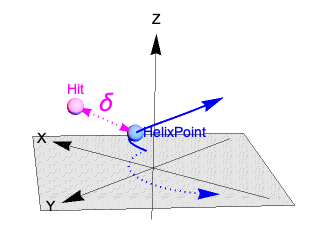
\includegraphics[width=200 pt]{Helix}
				\put(-180,120){
					\large (a)
				}
			}
			\put(200,0){
				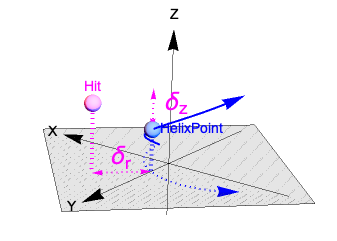
\includegraphics[width=200 pt]{Planar}
			\put(-180,120){
					\large (b)
				}
			}
		\end{picture}
		\caption{}\label{Rep}
	\end{figure}
	\section{Position Residual Comparison with HypTPC Data}
		\begin{figure}[h]
		\centering
		\begin{picture}(400,180)
			\put(0,0){
				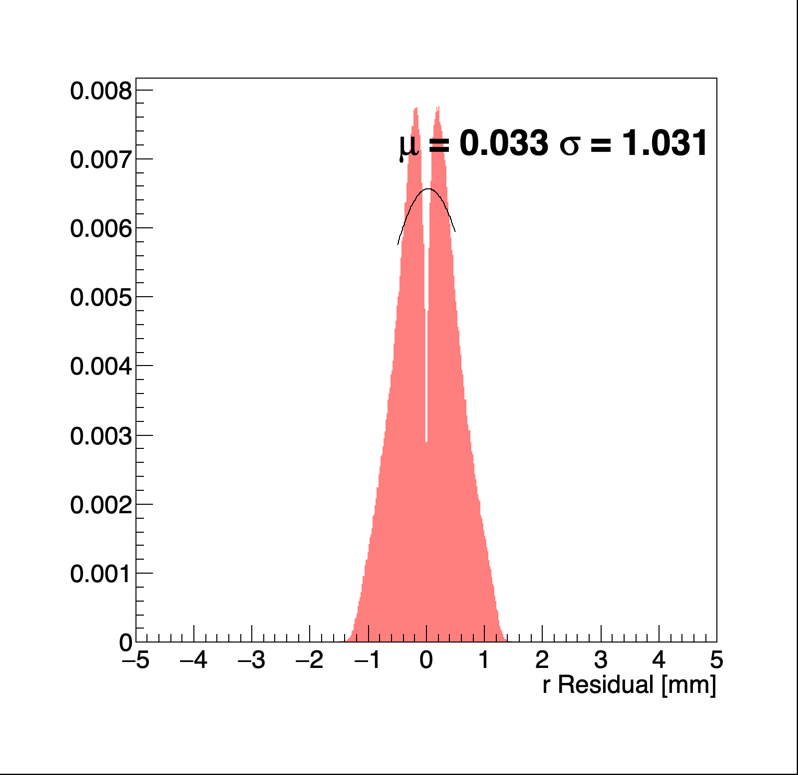
\includegraphics[width=200 pt]{ResR_Helix}
				\put(-160,150){
					\large (a)
				}
			}
			\put(200,0){
				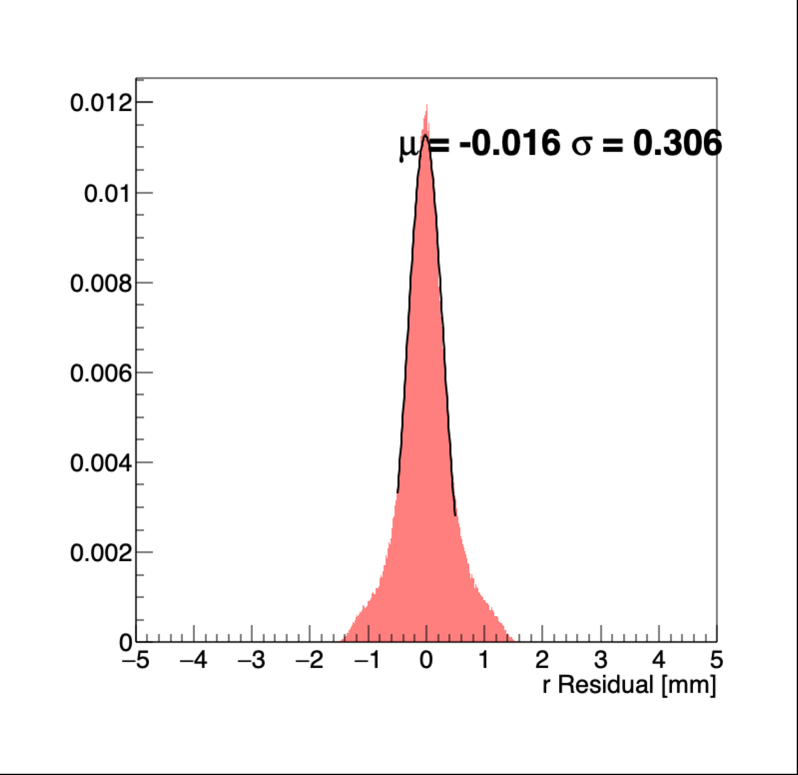
\includegraphics[width=200 pt]{ResR_Planar}
				\put(-160,150){
					\large (b)
				}
			}
		\end{picture}
		\caption{}\label{Resi}
	\end{figure}
	Figure \ref{Resi} compares the radial residuals obtained using (a) the PoC Method and (b) the MRD method for scattered $\pi$ tracks from a $^{12}$C target in a 1T B-field. As discussed in the previous section, the PoC method minimizes the total squared distance, $\delta_r^2+\delta_T^2$, so the radial component $\delta_r$ alone is not necessarily minimized. This results in the dip structure observed in (a).
	\section{Position Resolution}
	\subsection{Radial Resolution}
	To be written... Check \cite{TPCRes}
	\subsection{Vertical Resolution}
	To be written...
	\section{Momentum Resolution in HypTPC Beamthrough Analysis}
	To be written...
	\begin{thebibliography}{}
		\bibitem{TPCRes}
		TPC Spatial Resolution Study from W.S. Jung\\
		\href{https://lambda.phys.tohoku.ac.jp/hyptpc-wiki/lib/exe/fetch.php?media=document:analysis:tpcspatialresolution.pdf}%
		{https://lambda.phys.tohoku.ac.jp/hyptpc-wiki/lib/exe/fetch.php?media=document:analysis:tpcspatialresolution.pdf}
	\end{thebibliography}
\end{document}
